\documentclass{standalone}

\usepackage{amssymb}
\usepackage{amsthm}
\usepackage{amsmath}


\usepackage{tikz}
\usetikzlibrary{shapes,backgrounds,calc,patterns}
\usepackage{venndiagram}


\begin{document}
    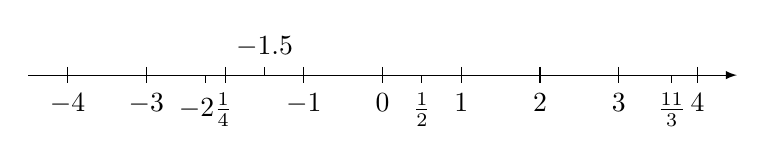
\begin{tikzpicture}
\draw[-latex] (-4.5,0) -- (4.5,0) ;
\foreach \x in  {-4,-3,-2,-1,0,1,2,3,4}
\draw[shift={(\x,0)},color=black] (0pt,3pt) -- (0pt,-3pt);
\foreach \x in {-4,-3,-1,0,1,2,3,4}
\draw[shift={(\x,0)},color=black] (0pt,0pt) -- (0pt,-3pt) node[below] {\(\x\)};
\draw[shift={(.5,0)},color=black] (0pt,0pt) -- (0pt,-3pt) node[below] {\( \frac{1}{2} \)};
\draw[shift={(3.67,0)},color=black] (0pt,0pt) -- (0pt,-3pt) node[below] {\( \frac{11}{3} \)};
\draw[shift={(-2.25,0)},color=black] (0pt,0pt) -- (0pt,-3pt) node[below] {\( -2\frac{1}{4} \)};
\draw[shift={(-1.5,0)},color=black] (0pt,0pt) -- (0pt,3pt) node[above] {\( -1.5 \)};
\end{tikzpicture}
\end{document}